\documentclass[border=3pt]{standalone}

\usepackage{tikz}
\usetikzlibrary{arrows.meta, decorations.pathreplacing}
\usepackage[T1]{fontenc}
\usepackage{newtxtext,newtxmath}

% OpenTikZ light palette (color-blind-friendly Okabe-Ito).
\definecolor{otblue}{HTML}{0072B2}
\definecolor{otorange}{HTML}{E69F00}
\definecolor{otteal}{HTML}{009E73}
\definecolor{otpurple}{HTML}{CC79A7}
\definecolor{otgray}{HTML}{5A5A5A}

\begin{document}
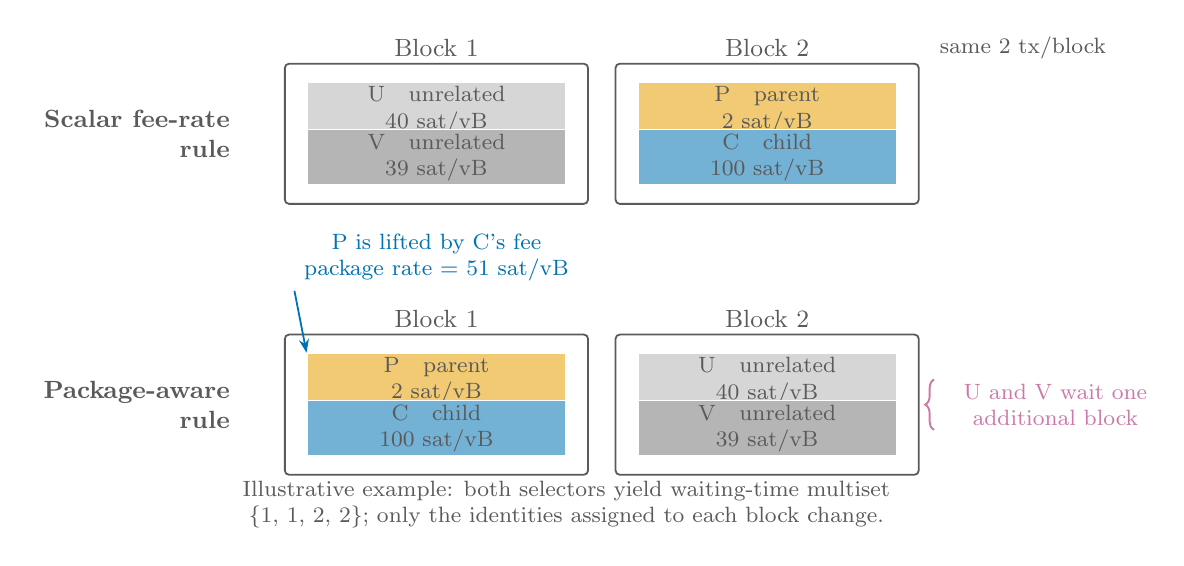
\begin{tikzpicture}[
  x=1cm,
  y=1cm,
  frame/.style={draw=otgray, line width=0.65pt, rounded corners=1.5pt,
                minimum width=3.85cm, minimum height=1.78cm},
  tx/.style={draw=white, line width=0.55pt, minimum width=3.28cm,
             minimum height=0.54cm, align=center, inner sep=1.5pt,
             font=\footnotesize\rmfamily, text=otgray},
  rule/.style={font=\bfseries\small\rmfamily, text=otgray, align=right,
               text width=2.45cm},
  block/.style={font=\small\rmfamily, text=otgray, align=center},
  note/.style={font=\footnotesize\rmfamily, align=center},
  leader/.style={-{Stealth[length=1.7mm]}, line width=0.65pt},
]

% Parameters: two policy rows, two blocks per row, equal transaction capacity.
\def\blockone{-1.65}
\def\blocktwo{2.55}
\def\scalarrow{1.82}
\def\packagerow{-1.62}

% Scalar fee-rate rule.
\node[rule, anchor=east] at (-4.15,\scalarrow) {Scalar fee-rate\\rule};
\node[block] at (\blockone,2.91) {Block 1};
\node[block] at (\blocktwo,2.91) {Block 2};
\node[frame] (scalar-block-one) at (\blockone,\scalarrow) {};
\node[frame] (scalar-block-two) at (\blocktwo,\scalarrow) {};
\node[tx, fill=otgray!25] at (\blockone,\scalarrow+0.30) {U\quad unrelated\\40 sat/vB};
\node[tx, fill=otgray!45] at (\blockone,\scalarrow-0.30) {V\quad unrelated\\39 sat/vB};
\node[tx, fill=otorange!55] at (\blocktwo,\scalarrow+0.30) {P\quad parent\\2 sat/vB};
\node[tx, fill=otblue!55] at (\blocktwo,\scalarrow-0.30) {C\quad child\\100 sat/vB};

% Package-aware rule.
\node[rule, anchor=east] at (-4.15,\packagerow) {Package-aware\\rule};
\node[block] at (\blockone,-0.53) {Block 1};
\node[block] at (\blocktwo,-0.53) {Block 2};
\node[frame] (package-block-one) at (\blockone,\packagerow) {};
\node[frame] (package-block-two) at (\blocktwo,\packagerow) {};
\node[tx, fill=otorange!55] (package-parent) at (\blockone,\packagerow+0.30) {P\quad parent\\2 sat/vB};
\node[tx, fill=otblue!55] (package-child) at (\blockone,\packagerow-0.30) {C\quad child\\100 sat/vB};
\node[tx, fill=otgray!25] (unrelated-u) at (\blocktwo,\packagerow+0.30) {U\quad unrelated\\40 sat/vB};
\node[tx, fill=otgray!45] (unrelated-v) at (\blocktwo,\packagerow-0.30) {V\quad unrelated\\39 sat/vB};

% One capacity note applies to both rows.
\node[note, anchor=west, text=otgray] at (4.62,2.91) {same 2 tx/block};

% Explain the package premium in the open space between policy rows.
\node[note, text=otblue] (package-note) at (\blockone,0.25)
  {P is lifted by C's fee\\package rate = 51 sat/vB};
\draw[leader, draw=otblue] (package-note.south west) -- (package-parent.north west);

% Mark both displaced transactions with one bracket and a clear side label.
\draw[decorate, decoration={brace, amplitude=3.2pt, mirror}, draw=otpurple,
      line width=0.7pt] (4.67,-1.30) -- (4.67,-1.94);
\node[note, anchor=west, text=otpurple] at (4.92,\packagerow)
  {U and V wait one\\additional block};

\node[font=\footnotesize\rmfamily, text=otgray, align=center]
  at (0,-2.89)
  {Illustrative example: both selectors yield waiting-time multiset\\
   \{1, 1, 2, 2\}; only the identities assigned to each block change.};

\end{tikzpicture}
\end{document}
